\section{Process Analysis}
\label{process-analysis}

\paragraph{Doing research and \project{} data}
When doing research in the medical domain a well known workflow is often used, Nwogu \cite{nwogu} has formally described and defined this.
Figure \ref{fig:research-workflow} shows the simplification of this workflow.
Note: the data acquisition block stands for the execution of acquisition methods, which in their turn belong to the method block.

Clinical research (\eg{} trials) is well suited to follow this workflow, each step can be executed in turn and data acquisition is often the most time consuming part.
However, with the rise of cheap disk space and big data this does not have to be true.
Research data of high quality and trustworthiness can be stored and re-used endlessly.
This is also the point of the \project{}, where considerable time has been spend on gathering data.

\begin{figure}[hb]
	\centering
	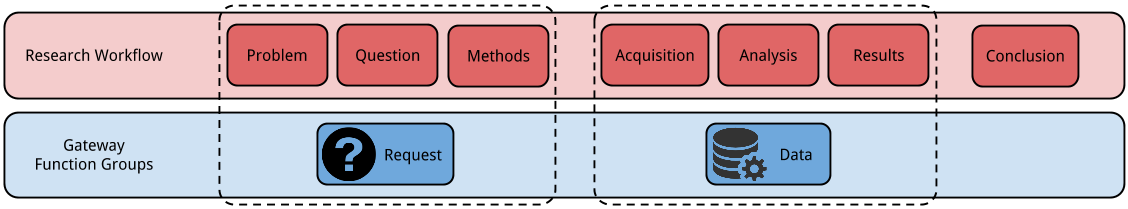
\includegraphics[width=1.0\linewidth]{images/research-workflow}
	\caption{
		This figure shows the often used research workflow in the medical domain, it is based on the structure described in Nwogu \cite{nwogu}.
		The workflow building blocks are mapped by the identified system function groups.
	}
	\label{fig:research-workflow}
\end{figure}

\paragraph{System functionality concept}
Restricting the use of data to one user is undesirable, therefore good data management has to be applied to enable re-use.
The initial system idea (seed) was for a data management system with data-centred functions, \eg{} request, upload, download, search.
These are represented in figure \ref{fig:research-workflow} with the blocks `request' and `data'.
With these functions a broad part of the research workflow will be supported, missing the conclusion (\ie{} publication) step.

\begin{figure}[t]
	\centering
	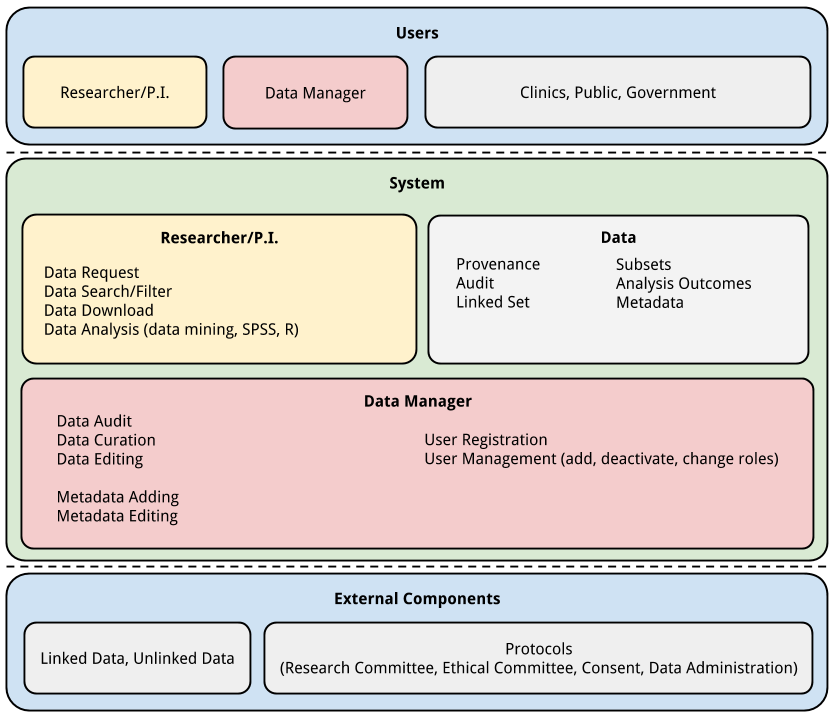
\includegraphics[width=1.0\linewidth]{images/brainstorm-before}
	\caption{
		Initial idea for the \ivfsystem{}, encompassing data and user management.
		External services are provided and outside of the scope of this paper.
		Two direct users and several external users are planned each with their specific set of functions.
		Data listed is either available at initialisation of the system or is generated during execution.
	}
	\label{fig:brainstorm-before}
\end{figure}

Figure \ref{fig:brainstorm-before} describes the full view of the seed, the function groups are expanded into: users, external services, data, and functions.
The external services are of influence on the system but are outside of the scope of this paper.
Meaning that data and protocols (necessary for lawful execution of the system) are already provided.
From the provided data unlinked data is \project{} data split into clinics and PRN, where linked data are the matched rows from both.
Projected direct users are researchers and data managers.
Furthermore, external parties (clinics, public, government) might be interested in statistics of the system and its data, \eg{} aggregated and anonymised analysis outcomes.

Functions for each of the users encompass data management and user management.
Data functions meaning mutations of the raw \project{} data, where metadata is metadata of this raw data.
The data block refers to data being stored in the system at initialisation and during execution.
The linked set (\ie{} raw data) is an initialisation input of the system.
Other items are generated during execution, \eg{} subsets are created after a data request is granted which also results in provenance data, etc.